\documentclass{article}
\usepackage[a4paper, top=3cm, bottom=2.5cm, left=2.5cm, right=2.5cm]{geometry} % Ajuste de márgenes
\usepackage[spanish]{babel}
\usepackage[utf8]{inputenc}
\usepackage{tabularx}
\usepackage{tikz}
\usepackage{titling}
\usepackage{graphicx}
\usepackage{fancyhdr}
\usepackage{amsmath}
\usepackage{amssymb}
\usepackage{multicol}
\usepackage{cancel}
\usepackage{pgfplots}
\usepackage{hyperref}
\usepackage{bookmark}
\pgfplotsset{compat=1.18}
\usepackage{titlesec} % Para personalizar títulos
\usepackage{tocloft}  % Para mejorar el índice
\usepackage{setspace} % Para controlar el espaciado

\usepackage{xcolor}
\usepackage{enumitem}

\definecolor{headerblue}{RGB}{50,90,140}
\definecolor{responsegray}{RGB}{80,80,80}



% Configuración de Fancyhdr para encabezados y pies de página
\pagestyle{fancy}
\fancyhf{}
\fancyhead[L]{
\includegraphics[width=2cm]{assets/logo-utp.png}}
\fancyhead[R]{\textbf{Diseño de Productos y Servicios}}

\fancyfoot[R]{\thepage} % Número de página alineado a la derecha

% Ajustes de espaciado entre párrafos y márgenes superiores
\setlength{\parskip}{1.5em}
\setlength{\parindent}{0pt}
\setlength{\headheight}{17.26935pt} % Altura del encabezado
\addtolength{\topmargin}{-2.26935pt} % Compensar el aumento de la altura del encabezado
\setlength{\textheight}{23cm}  % Ajusta el alto del texto

% Definición de comandos personalizados
\newcommand{\SubItem}[1]{
    {\setlength\itemindent{15pt} \item[-] #1}
}

% Título del documento con mejor control de espaciado
\title{
  
\includegraphics[width=5cm]{./assets/logo-utp.png} \\
  \vspace{1cm}
  \textbf{Universidad Tecnológica del Perú} \\
  \vspace{2cm}
  \textbf{Detectives de Benchmarking y Tu propuesta de Valor.} \\
  \vspace{1cm}
  \large \textbf{Para el curso de Diseño de Productos y Servicios.}
}
\author{
  \textbf{Luis Huatay Salcedo.} \\
  \textbf{Garcia Chumpitaz Cindel Roxell.} \\
  \textbf{Díaz Benítez, Fernando Raúl.} \\
  \textbf{Quispe Fernandez, Bryan Alexander.}
}


\begin{document}
\maketitle
\begin{center}
  Sección 44698
\end{center}
\thispagestyle{empty}
\begin{center}
  Mg. Marcos Teodoro Yerren Huima  
\end{center}
\restoregeometry

% \newpage

% \begin{center}
%   \textbf{\Large Índice}
% \end{center}
% \vspace{0.5cm} % Espacio entre título y contenido

% \begin{spacing}{1.15} % Espaciado personalizado para mayor legibilidad
%   \noindent
%   \begin{enumerate}
%     \item Introducción
%   %   \item Problemática
%   %   \item Objetivo general
%   %   \begin{enumerate}
%   %     \item Objetivos específicos
%   %   \end{enumerate}
%   %   \item Términos estadísticos
%   %   \item Recolección de información
%     \end{enumerate}
% \end{spacing}

\newpage


%-------------------------------------------------
% Perfil del usuario
%-------------------------------------------------
\section{Detectives de Benchmarking}

En esta actividad aplicaremos la técnica de benchmarking para identificar oportunidades de mejora en la experiencia de usuario de una aplicación digital. Para ello, realizaremos una comparación entre productos.

\subsection*{Producto:}
\textit{\textbf{Sala de estudios SS }}

Dirigido a estudiantes enfocado en el servicio de la reserva de salas de estudio. La aplicación permite a los estudiantes reservar salas de estudio en la universidad, facilitando la gestión del tiempo y el espacio para el estudio.

\subsection{Cuadro comparativo de productos}

Competencia: \textbf{Starbucks} - \textbf{Bembos}

\begin{table}[ht]
  \centering
  \scriptsize
  % Ajuste automático de ancho con tabularx
  \begin{tabularx}{\textwidth}{|>{\raggedright\arraybackslash}X|>{\raggedright\arraybackslash}X|>{\raggedright\arraybackslash}X|>{\raggedright\arraybackslash}X|>{\raggedright\arraybackslash}X|>{\raggedright\arraybackslash}X|}
  \hline
  \textbf{Producto} & \textbf{Público objetivo} & \textbf{Principales funciones} & \textbf{Fortalezas} & \textbf{Debilidades} & \textbf{Valor diferenciador} \\
  \hline
  Sala de estudios & Estudiantes  & Reserva inteligente por disponibilidad  & Solicitud de servicios externos; gratuito  & Salas limitadas; aire acondicionado compartido; espacio reducido  & Gratis frente a la competencia  \\
  \hline
  Starbucks & Público general  & Venta de productos y servicio de cafetería  & Atención rápida; ambiente atractivo  & Sin pizarras; sin computadoras; internet lento  & Experiencia cuidada y consistente  \\
  \hline
  Bembos & Público general  & Comida rápida; opción de almuerzo  & Precios accesibles; menú variado  & Ambiente ruidoso; no propicio para el estudio  & Espacios recreativos para niños  \\
  \hline
  \end{tabularx}
  \caption{Comparación de productos y su propuesta de valor ajustada}
  \label{tab:comparacion-productos}
  \end{table}
  
\newpage

\section{Actividad 2: “Tu Propuesta, Tu Valor”}

\begin{description}[leftmargin=2cm,style=nextline]
  \item[Para] \textbf{estudiantes}
  \item[que necesitan] \textbf{salas / espacio de estudios}
  \item[nuestra solución es] \textbf{sistema de reservas}
  \item[que ofrece] \textbf{reservar salas de estudio}
  \item[a diferencia de] \textbf{mayor cantidad de servicios}
  \item[porque] \textbf{enfocado a estudiantes}
\end{description}

\noindent\textbf{Producto Final:}

Nuestro producto final va dirigido a estudiantes universitarios que necesitan acceder y reservar espacios de estudio. Nuestra solución es un sistema de reservas en línea que ofrece confirmación instantánea y gestión de disponibilidad en tiempo real, a diferencia de las plataformas genéricas con múltiples servicios dispersos, porque está diseñado específicamente para optimizar la experiencia de estudio.

\begin{figure}[ht]
  \centering
  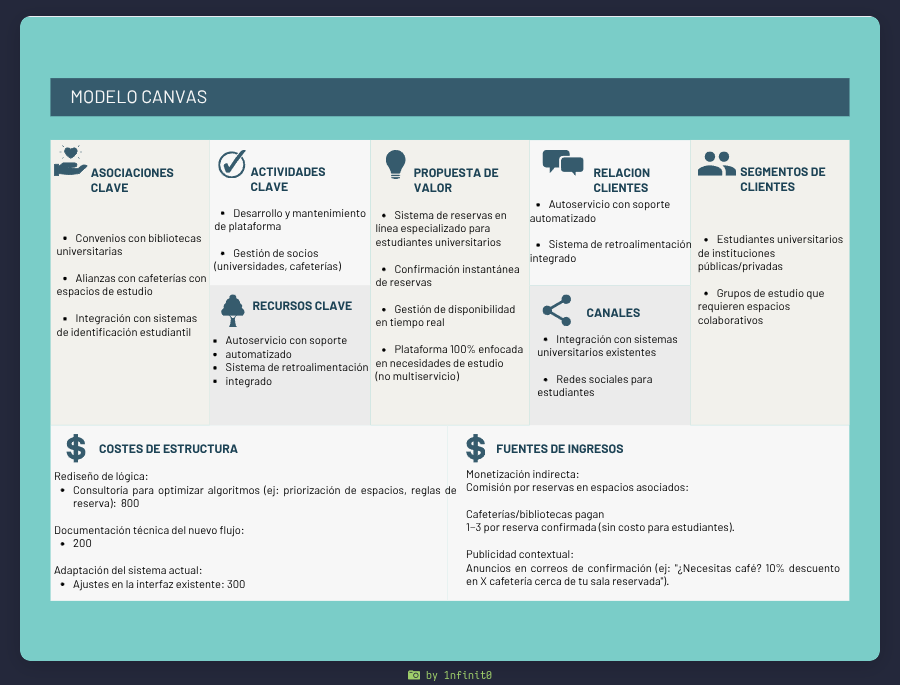
\includegraphics[width=0.8\textwidth]{assets/lean.png}
  \caption{Modelo de Lean Canvas}
  \label{fig:example-image}
\end{figure}

\end{document}